\chapter{Results}

In this chapter we will present the results of the experiments \nameExperimentI{} and \nameExperimentII{}, along with a discussion of the impact on the lift and similarity distributions of these experiments relative to the OT without the clustering.

\section{Experiment \nameExperimentI}

As seen on \ref{ch:experiment-i} this experiment was the one that creates sub-runs of the OT for each cluster in the portfolio. Also, it had to be created some heuristics to deal with clusters that did not have enough data to run. Using the "manual clustering", as discussed on \ref{ch:cluster-algorithm} the summary of the lift gain (how much the lift on the first decile increased or decreased relative to the OT without clustering) is presented on Table \ref{table:lift_gain_exp-i}. Figure \ref{fig:lift-hist-plot-exp-i} shows another perspective for this data through a histogram, excluding the outliers studies.

The cells are colored to better understand the gains. The dark colors (green and red) represent a considerable positive or negative gain, the light colors a slight positive or negative gain. The white, represent that the lift did not change. Finally, the orange ones are the outliers which were defined using the interquartile range rule \cite{upton1996understanding}. 

\begin{table}[!ht]
\centering
\begin{adjustbox}{max width=7cm}
\begin{tabular}{|c|c|c|c|}
\hline
\textbf{Study} & \textbf{Lift Gain (\%)}        & \textbf{Study} & \textbf{Lift Gain (\%)}        \\ \hline
1              & \cellcolor[HTML]{ff514d}-12,09 & 15             & \cellcolor[HTML]{ff514d}-13,26 \\ \hline
2              & \cellcolor[HTML]{009901}16,67  & \textbf{16}    & \cellcolor[HTML]{ff514d}-20,00 \\ \hline
3              & \cellcolor[HTML]{00c901}0,89   & \textbf{17}    & \cellcolor[HTML]{ffccc9}-4,28  \\ \hline
4              & 0,00                           & 18             & \cellcolor[HTML]{ff514d}-13,06 \\ \hline
5              & \cellcolor[HTML]{ffccc9}-0,14  & 19             & \cellcolor[HTML]{ff514d}-15,42 \\ \hline
6              & \cellcolor[HTML]{ff514d}-17,28 & 20             & \cellcolor[HTML]{00c901}0,57   \\ \hline
7              & \cellcolor[HTML]{ff514d}-12,44 & \textbf{21}    & \cellcolor[HTML]{ff514d}-33,95 \\ \hline
\textbf{8}     & \cellcolor[HTML]{ffccc9}-5,17  & 22             & 0,00                           \\ \hline
\textbf{9}     & \cellcolor[HTML]{ff514d}-27,78 & 23             & \cellcolor[HTML]{ff514d}-28,16 \\ \hline
\textbf{10}    & \cellcolor[HTML]{009901}6,25   & 24             & \cellcolor[HTML]{ffce93}200,01 \\ \hline
11             & \cellcolor[HTML]{ff514d}-17,75 & \textbf{25}    & \cellcolor[HTML]{ff514d}-12,77 \\ \hline
12             & \cellcolor[HTML]{ffccc9}-1,01  & 26             & \cellcolor[HTML]{ff514d}-29,35 \\ \hline
13             & \cellcolor[HTML]{ff514d}-6,93  & 27             & \cellcolor[HTML]{ffccc9}-0,08  \\ \hline
14             & \cellcolor[HTML]{ffccc9}-1,16  &                &                                \\ \hline
\end{tabular}
\end{adjustbox}
\caption{Summary of the first-decile lift gains for Experiment \nameExperimentI}
\label{table:lift_gain_exp-i}
\end{table}

\begin{figure}[!ht]
   \centering
   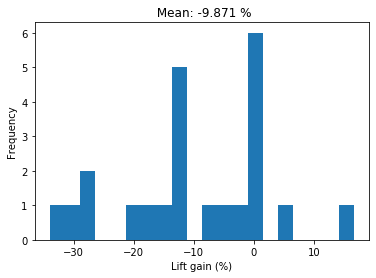
\includegraphics[width=8cm]{fig/ch4-lift-hist-plot-exp-i.png}
   \caption{Histogram plot of the studies' lift gain for experiment \nameExperimentI{}. Source: Author}
   \label{fig:lift-hist-plot-exp-i}
\end{figure}

There are also some studies that are bolded. They represent the studies that brought up the hypothesis of this work, as discussed at the Introduction, they had two or more high density areas on the similarity distribution plot, meaning that, they can have more than one profile on their portfolio.

We can see that only five studies had positive impact on the lift, and one of them is an outlier. The majority of the studies had a negative impact, six of them were sightly negative and fourteen worsened the lift considerably. It is important to notice that two studies did not present any changes on the lift with the clustering. The overall mean lift gain for \nameExperimentI{} is $-9,871 \%$.


\section{Experiment \nameExperimentII{}}

Now for the second experiment, which was the simple use of the clustering information as another feature. Using the same color scheme as Table \ref{table:lift_gain_exp-i}, Table \ref{table:lift_gain_exp-ii} shows the summary of the lift gains for the experiment \nameExperimentII{}. Figure \ref{fig:lift-hist-plot-exp-ii} this data in a histogram (without outliers studies).

\begin{table}[!ht]
\centering
\begin{adjustbox}{max width=7cm}
\begin{tabular}{|c|c|c|c|}
\hline
\textbf{Study} & \textbf{Lift Gain (\%)}        & \textbf{Study} & \textbf{Lift Gain (\%)}        \\ \hline
1              & \cellcolor[HTML]{00c901}4,40   & 15             & \cellcolor[HTML]{00c901}0,46   \\ \hline
2              & \cellcolor[HTML]{ff514d}-8,33  & \textbf{16}    & \cellcolor[HTML]{ff514d}-6,58  \\ \hline
3              & \cellcolor[HTML]{009901}23,65  & \textbf{17}    & \cellcolor[HTML]{ffce93}-46,08 \\ \hline
4              & 0,00                           & 18             & \cellcolor[HTML]{ffccc9}-1,87  \\ \hline
5              & \cellcolor[HTML]{00c901}1,49   & 19             & \cellcolor[HTML]{00c901}3,58   \\ \hline
6              & \cellcolor[HTML]{ffce93}-28,33 & 20             & \cellcolor[HTML]{ff514d}-11,28 \\ \hline
7              & \cellcolor[HTML]{009901}12,50  & \textbf{21}    & \cellcolor[HTML]{ffccc9}-2,64  \\ \hline
\textbf{8}     & \cellcolor[HTML]{009901}16,84  & 22             & \cellcolor[HTML]{00c901}1,23   \\ \hline
\textbf{9}     & \cellcolor[HTML]{009901}12,80  & 23             & \cellcolor[HTML]{ffccc9}-0,14  \\ \hline
\textbf{10}    & \cellcolor[HTML]{009901}18,59  & 24             & \cellcolor[HTML]{ffce93}300,02 \\ \hline
11             & \cellcolor[HTML]{ff514d}-7,84  & \textbf{25}    & \cellcolor[HTML]{00c901}4,90   \\ \hline
12             & \cellcolor[HTML]{ffccc9}-0,15  & 26             & \cellcolor[HTML]{ffccc9}-0,77  \\ \hline
13             & \cellcolor[HTML]{00c901}0,68   & 27             & \cellcolor[HTML]{00c901}1,21   \\ \hline
14             & \cellcolor[HTML]{009901}7,30   &                &                                \\ \hline
\end{tabular}
\end{adjustbox}
\caption{Summary of the first-decile lift gains for Experiment \nameExperimentII}
\label{table:lift_gain_exp-ii}
\end{table}

We can see that, differently from \nameExperimentI{}, the majority of the studies had positive gain (16 studies, to be exactly). Only four studies were considerably worse on the lift gain and five sightly worse, a total of nine studies. Only one study did not present any change to the lift and, this time, four were outliers (two positives and two negatives). The mean lift gain for \nameExperimentII{} is $2,016 \%$.

\begin{figure}[!ht]
   \centering
   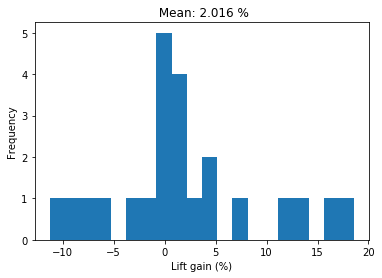
\includegraphics[width=8cm]{fig/ch4-lift-hist-plot-exp-ii.png}
   \caption{Histogram plot of the studies' lift gain for experiment \nameExperimentII{}. Source: Author}
   \label{fig:lift-hist-plot-exp-ii}
\end{figure}

\section{Similarity distributions}
\label{ch:simi-distis}

\newcommand{\simiDistWidth}{8cm}

Now let us look at some of the similarity distributions plots for both experiments. These plots will have three curves: the market similarity in green, the holdout set in orange, and the portfolio in blue. Each topic of this section will address a group represented by the colors in the lift gain summary tables. 

\subsection{Studies with no change to the lift}

In both experiments there were studies that did not lead to any change to the lift. Study 4 appeared on both. Figure \ref{fig:study-4-comparsion-exp-i} shows the similarity distribution plot for experiment \nameExperimentI{}, and \ref{fig:study-4-comparsion-exp-ii} for experiment \nameExperimentII{}. In both figures, the first row is the OT run without the clustering, and the second one is with the clustering. %This is a study with around 4600 companies on the portfolio (1100 are the Holdout set) and a market around 220 thousand companies, meaning that the portfolio corresponds to approximately $1,5\%$ of the companies on the study.

\begin{figure}[!ht]
   \centering
   
   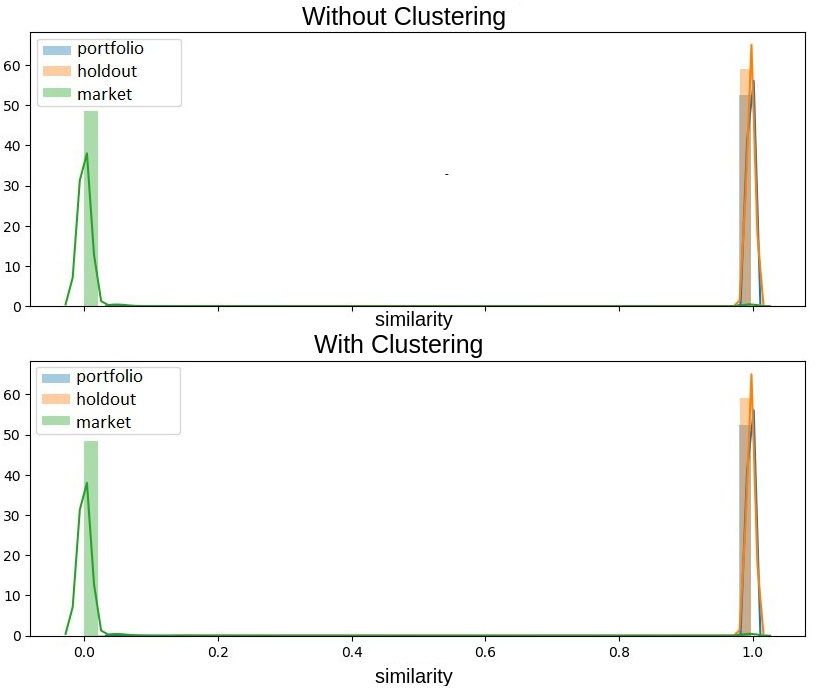
\includegraphics[width=8cm]{fig/ch4-study-4-comparsion-exp-i.png}
   \caption{Similarity distribution plot for Study 4 in experiment \nameExperimentI{}. Source: Author}
   \label{fig:study-4-comparsion-exp-i}

   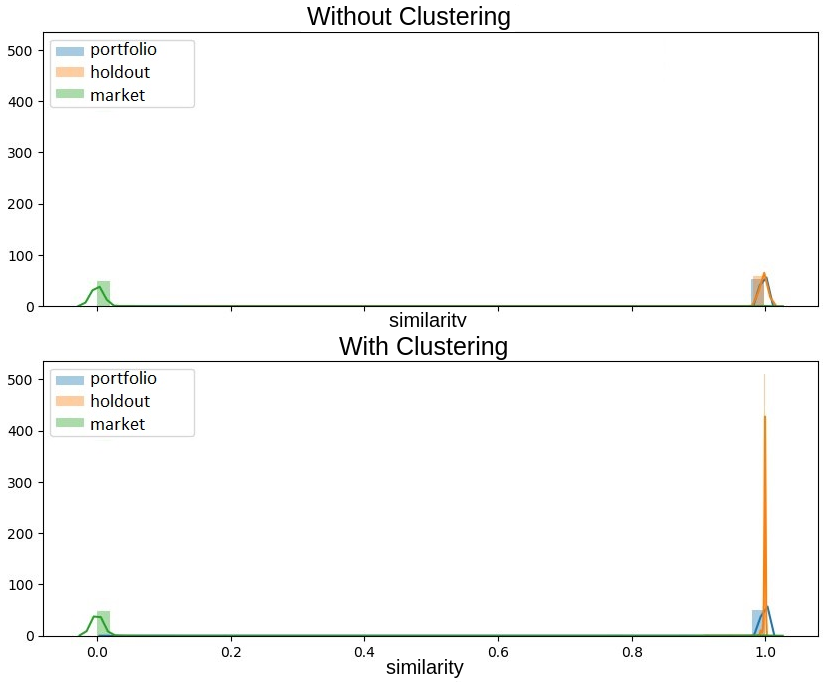
\includegraphics[width=8cm]{fig/ch4-study-4-comparsion-exp-ii.png}
   \caption{Similarity distribution plot for Study 4 for both experiments. Source: Author}
   \label{fig:study-4-comparsion-exp-ii}
\end{figure}

We can see that in experiment \nameExperimentI{} the similarity distributions with and without clustering are virtually the same. This is better understood when you look at the number of clusters in its portfolio. Figure \ref{fig:study-4-pca-plot} shows its PCA plot. There is only a single cluster on the portfolio, consequentially, the result of this cluster is the same regardless of using the clustering approach.

\begin{figure}[!ht]
   \centering
   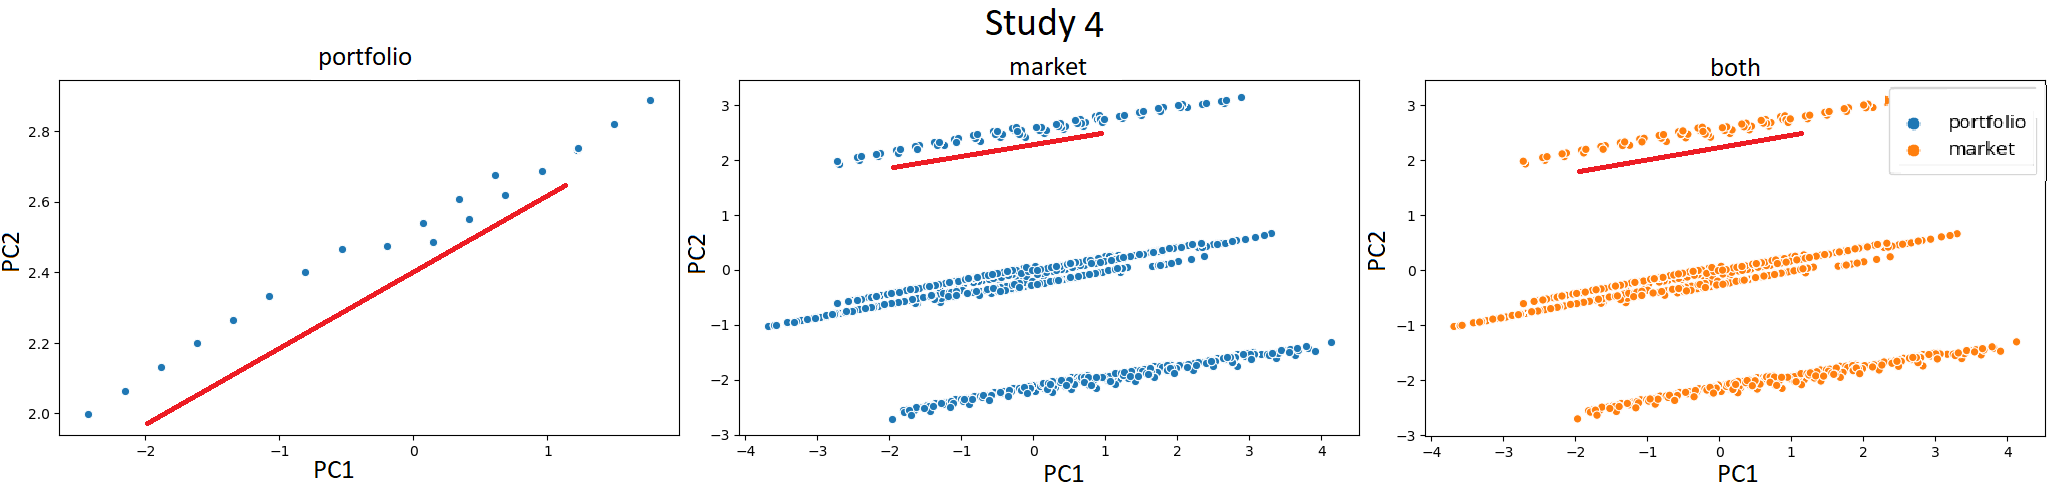
\includegraphics[width=\linewidth]{fig/ch4-study-4-pca-plot.png}
   \caption{PCA plot for Study 4. On the left there is just the portfolio, on the right both portoflio and market. Source: Author}
   \label{fig:study-4-pca-plot}
\end{figure}

In \nameExperimentII{}, however, there is a difference on the distributions between the with and without the clustering. Basically, the holdout set changed its distribution. In this experiment the OT scored these companies with really close scores, in other words, their standard deviation decreased. But, even though the scores of the companies (and possibly the ordering) of the holdout set changed, the lift kept the same because of how it is calculated. The same number of companies (of the holdout set) on the first decile occurred in the run without the clustering and in with the clustering, thus the value of the lift is the same for both runs.

Another study that had a zero lift gain was Study 22, in the \nameExperimentI{} experiment. Figure \ref{fig:study-22-clusters-simi-plot} shows the similarity distribution plots for the clusters' runs of this study.

\begin{figure}[!ht]
   \centering
   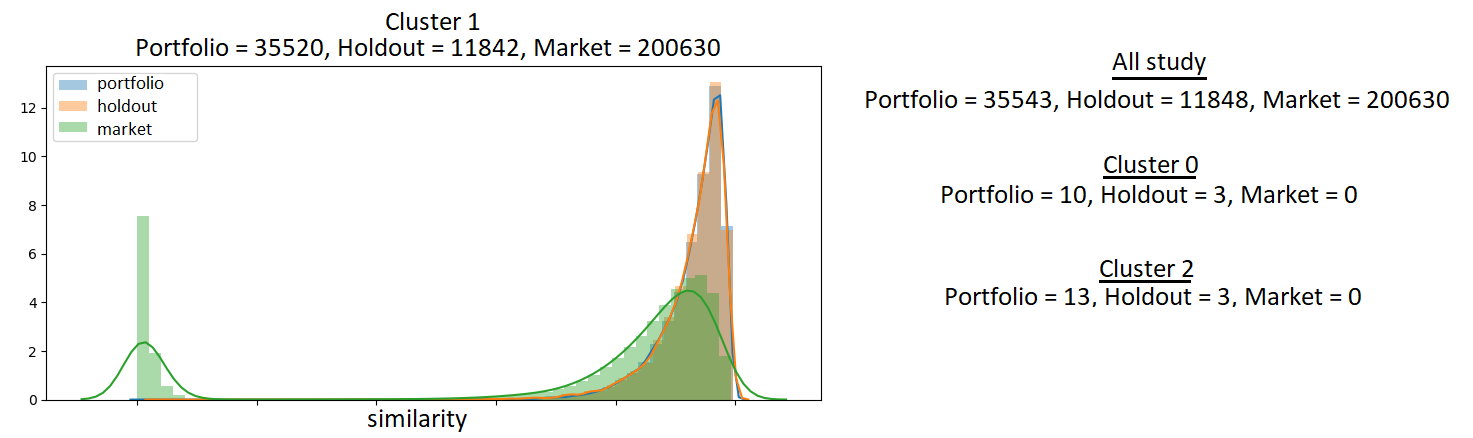
\includegraphics[width=8cm   ]{fig/ch4-study-22-clusters-simi-plot.png}
   \caption{Similarity distribution plot for the clusters' runs of Study 22 on experiment \nameExperimentI{}. Source: Author}
   \label{fig:study-22-clusters-simi-plot}
\end{figure}

Although this study has three clusters on the portfolio, only Cluster 1 has the minimum data to a valid run. Cluster 0 and Cluster 2 do not have companies on the Market, so the sixteen companies of the former and thirteen companies of the latter were discarded. Since they represent less than $0,001\%$ of the overall data of the study, the behavior is practically the same as Study 4, thus, for the same reason, the lift is the same for both runs (with and without clustering).

\subsection{Studies with marginal increase or decrease on the lift}
\label{ch:marginal-change}

Both experiments had studies that changed the lift in a minor way, positively and negatively. These studies improved or lowered the lift up to approximately $5\%$. They are presented in the light green and light red colors in tables previously mentioned. Experiment \nameExperimentI{} had two positives and five negatives. \nameExperimentII{} had seven and five, respectively.

All of these studies had the same prevalent behavior: the overall distributions of the three sets (portfolio, holdout, and market) before and after the clustering were almost the same. There is a small difference to the holdout distribution. Figures \ref{fig:study-5-marginal-increase-exp-2} and \ref{fig:study-12-marginal-decrease-exp-1} illustrate, respectively, examples of a small increase and decrease on the lift. In the former, the similarity distributions plot for Study 5 in experiment \nameExperimentII{}, and in the latter the same plot for Study 12 for experiment \nameExperimentI{}.

\begin{figure}[!ht]
   \centering
   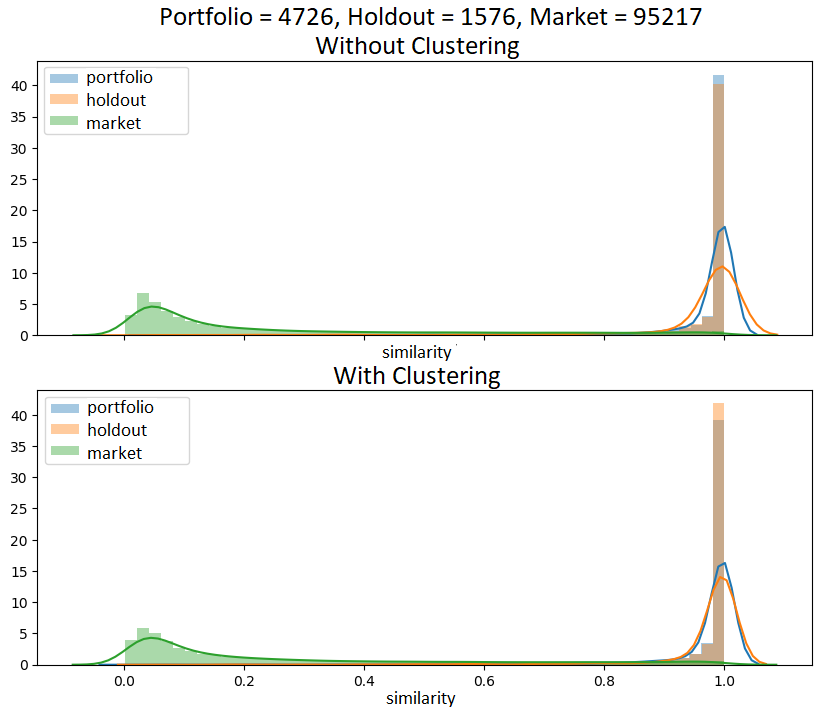
\includegraphics[width=8cm]{fig/ch4-study-5-marginal-increase-exp-2.png}
   \caption{Similarity distribution plot for Study 5 on experiment \nameExperimentII{}. An example of marginal increase on the lift. Source: Author}
   \label{fig:study-5-marginal-increase-exp-2}

   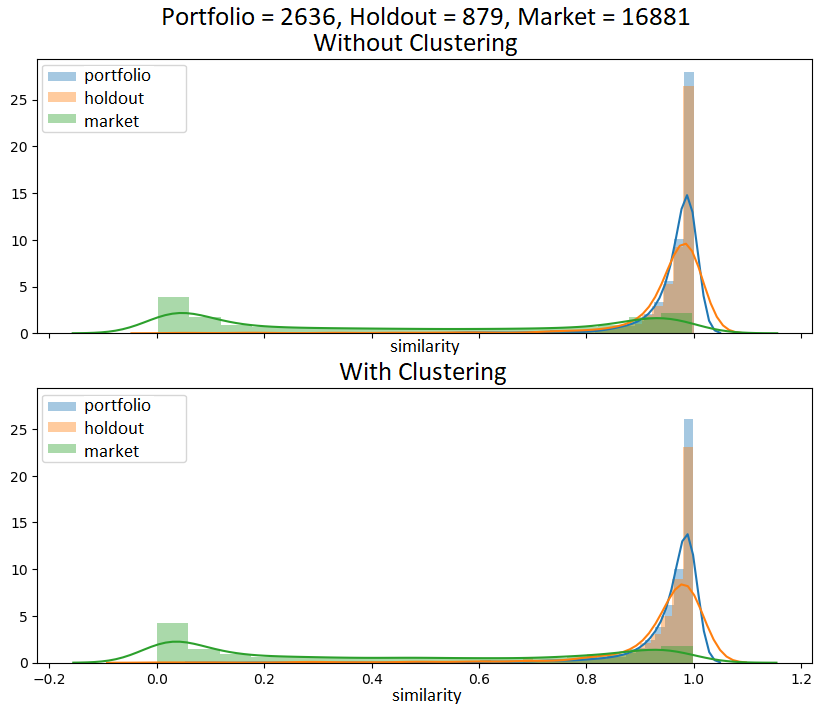
\includegraphics[width=8cm]{fig/ch4-study-12-marginal-decrease-exp-1.png}
   \caption{Similarity distribution plot for Study 12 on experiment \nameExperimentI{}. An example of marginal decrease on the lift. Source: Author}
   \label{fig:study-12-marginal-decrease-exp-1}
\end{figure}

We can notice that the peak near similarity $1,0$ of the holdout set goes from approximately $37,0$ to beyond $40,0$ in Figure \ref{fig:study-5-marginal-increase-exp-2}. The opposite happens in Figure \ref{fig:study-12-marginal-decrease-exp-1}, the peak goes from almost $25,0$ to $20,0$.

\subsection{Studies with considerable increase or decrease to the lift}
\label{ch:considerable-change}

Most of the studies on both experiments had more than $5\%$ variation to the lift (positive and negative). In \nameExperimentI{}, fourteen of them were negative and only Study 2 was positive. However, in experiment \nameExperimentII{}, five were positive and four were negative.

The behavior of the similarity distributions with the clustering follows the same idea as section \ref{ch:marginal-change}, but with more exacerbate results. Figure \ref{fig:study-8-considerable-increase-exp-2} shows the similarity distributions with and without clustering for Study 8 in experiment \nameExperimentII{}, which is an example of a considerable increase on lift. In contrast, Figure \ref{fig:study-9-considerable-decrease-exp-1} displays the same plot for Study 9 in experiment \nameExperimentI{}, an example of considerable decrease on the lift.

\begin{figure}[!ht]
   \centering
   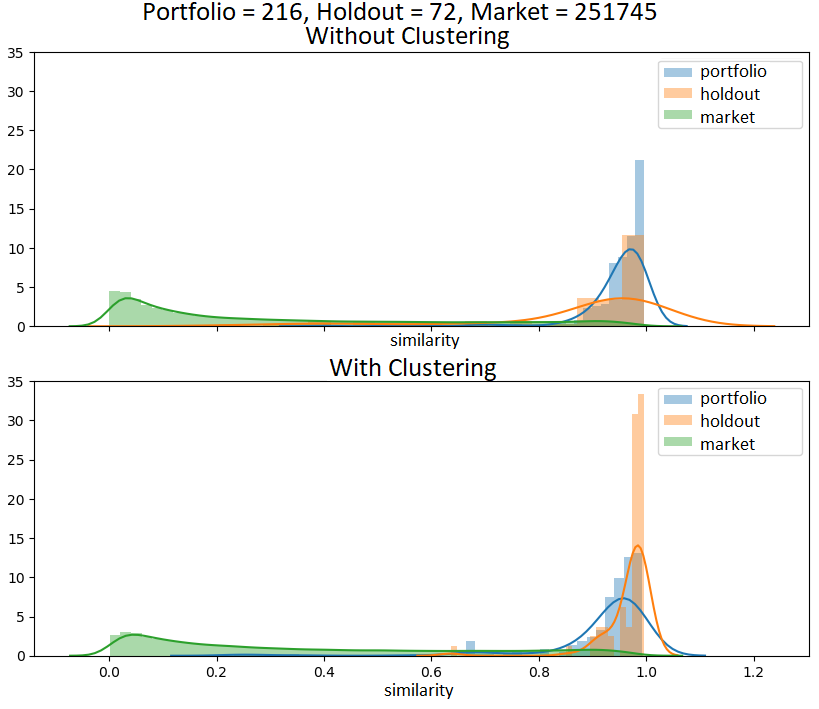
\includegraphics[width=8cm]{fig/ch4-study-8-considerable-increase-exp-2.png}
   \caption{Similarity distribution plot for Study 8 on experiment \nameExperimentII{}. An example of considerable increase on the lift. Source: Author}
   \label{fig:study-8-considerable-increase-exp-2}
\end{figure}

\begin{figure}[!ht]
   \centering
   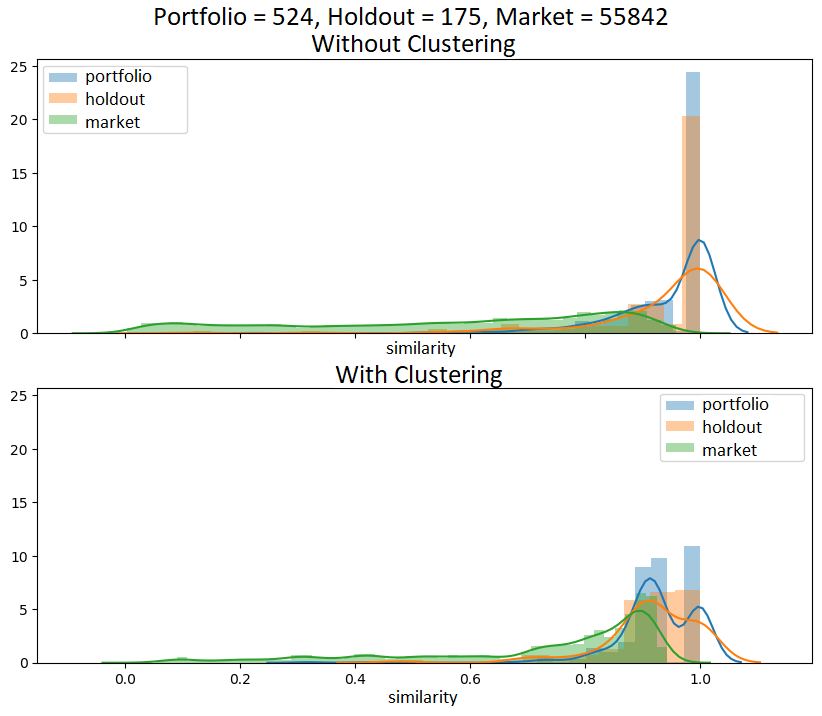
\includegraphics[width=8cm]{fig/ch4-study-9-considerable-decrease-exp-1.png}
   \caption{Similarity distribution plot for Study 9 on experiment \nameExperimentI{}. An example of considerable decrease on the lift. Source: Author}
   \label{fig:study-9-considerable-decrease-exp-1}
\end{figure}

Now the difference between the distributions, in these cases, is easier to spot. In Figure \ref{fig:study-8-considerable-increase-exp-2} we can see that the peak of the holdout set rose from $10,0$ to more than $30,0$. Consequentially, the curve became more thin, meaning that its variance decreased. The contrary to this, is showed on Figure \ref{fig:study-9-considerable-decrease-exp-1}. The peak of the holdout set distribution went from $20,0$ to less than $10,0$. Also, the portfolio distribution changed. Its single peak decreased by $15$ units, and it was splitted in two peaks, one near $0,9$ similarity and the other near similarity $1,0$. This demonstrates that the OT was better at scoring the portfolio near similarity $1,0$ without the clustering, which is the expected behavior. Moreover, the distribution of the market skewed to the right on this run, creating a high density area near $0,9$ similarity. 

\subsection{Outliers studies}
\label{ch:outliers}

Study 24 was clearly the outlier of all studies. It got more than $200\%$ increase on the lift in both Experiments. In experiment \nameExperimentII{} more three studies were considered outliers due to the interquartile range rule - the lower and upper bound in this experiment were $-14.77\%$ and $18.62\%$, respectively. These studies had similar shift on the distributions as seen in \ref{ch:considerable-change}. Hence, just Study 24 is presented here. Figure \ref{fig:outlier-study-24-exp-2} exhibits the similarity distribution plot of this study in \nameExperimentII{}, and Figure \ref{fig:outlier-study-24-lift-exp-2} its lift plots, which contains the lifts of all deciles of the runs with and without the clustering.

\begin{figure}[!ht]
   \centering
   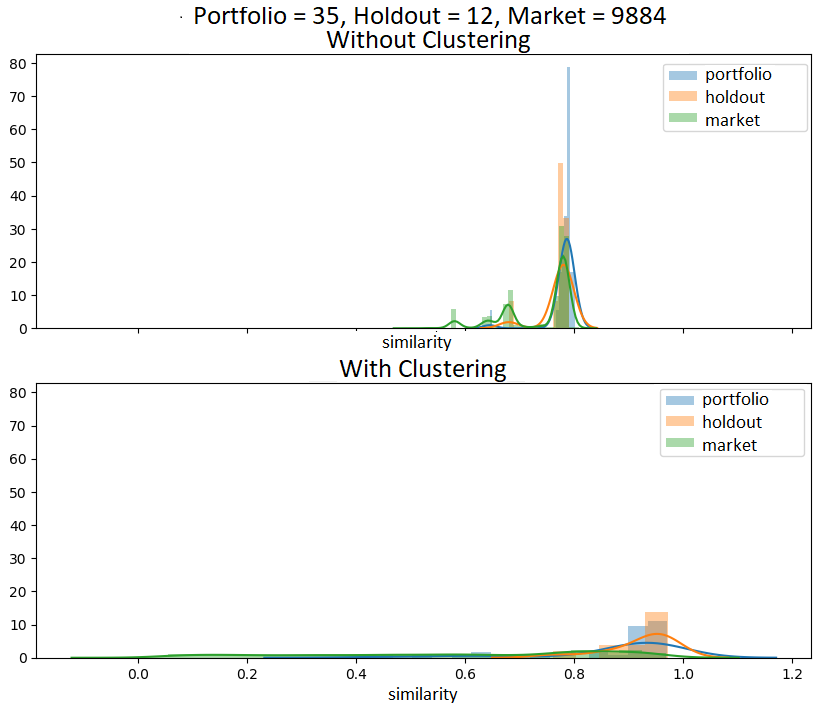
\includegraphics[width=8cm]{fig/ch4-outlier-study-24-exp-2.png}
   \caption{Similarity distribution plot for Study 24 on experiment \nameExperimentII{}. Source: Author}
   \label{fig:outlier-study-24-exp-2}
\end{figure}

The main aspect of this study is presented in Figure \ref{fig:outlier-study-24-exp-2}. The Figure shows unusual distributions with multiple modes (without clustering), the highest one located at similarity $0,8$. The OT failed to classify the portfolio of this study close similarity $1,0$. Moreover, the number of companies for each of the sets of the study is unbalanced. There are only 35 companies in the portfolio and twelve in the holdout set against a market with two orders of magnitude higher. This discrepancy can be one of the issues that led this study to have odd similarity distributions.

\begin{figure}[!ht]
   \centering
   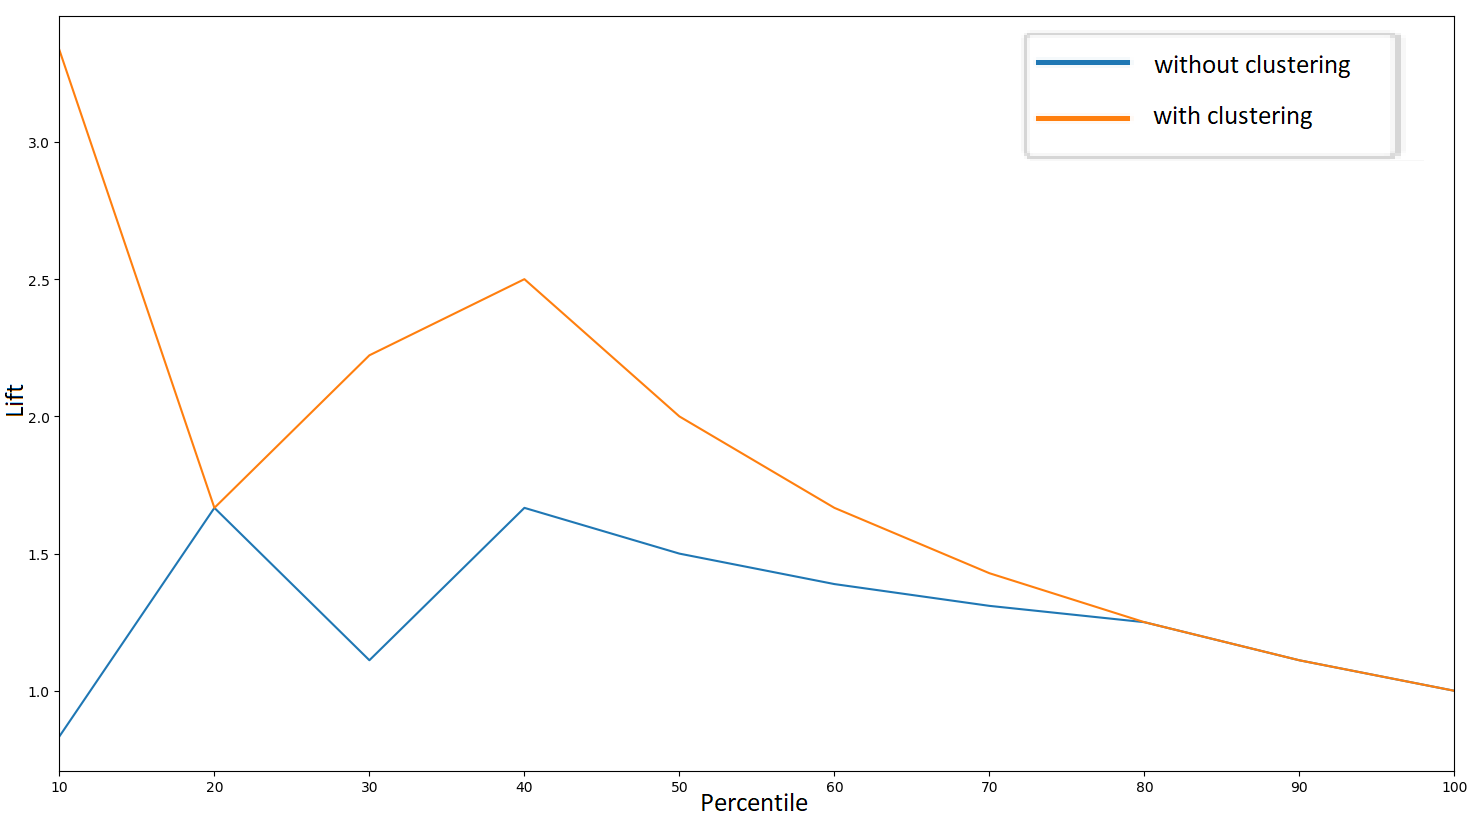
\includegraphics[width=8cm]{fig/ch4-outlier-study-24-lift-exp-2.png}
   \caption{Lift plot for Study 24 on experiment \nameExperimentII{}. Source: Author}
   \label{fig:outlier-study-24-lift-exp-2}
\end{figure}

This issue is reinforced when we look at Figure \ref{fig:outlier-study-24-lift-exp-2}. The expected shape of a lift curve is in the form of a decreasing exponential, in other words, the lift of the decile on the left is greater than the one in the right, but this is not what happens on both runs of the experiment for this study. In the run with the clustering the lift of the second decile is lower than the fourth one. On top of that, the lift of the first decile in the run without the clustering is lower than $1,0$. 

With the clustering, the distributions skewed to the right, with the holdout set being the closest to similarity $1,0$. This explains why the lift of the first decile increased over $200\%$ in the run with the clustering.

\subsection{Studies that had multiple profiles in its portfolio}

The last group of studies to be analyzed are the bolded ones in both tables (\ref{table:lift_gain_exp-i} and \ref{table:lift_gain_exp-ii}). These are the studies that sparked the idea of clustering the portfolio before running the OT. However, most of them did not had the expected behavior. Let us use one example that illustrate this result. Figure \ref{fig:bump-study-25} displays the similarity distributions plots for Study 25 for the runs in experiment \nameExperimentII{}. 

\begin{figure}[H]
   \centering
   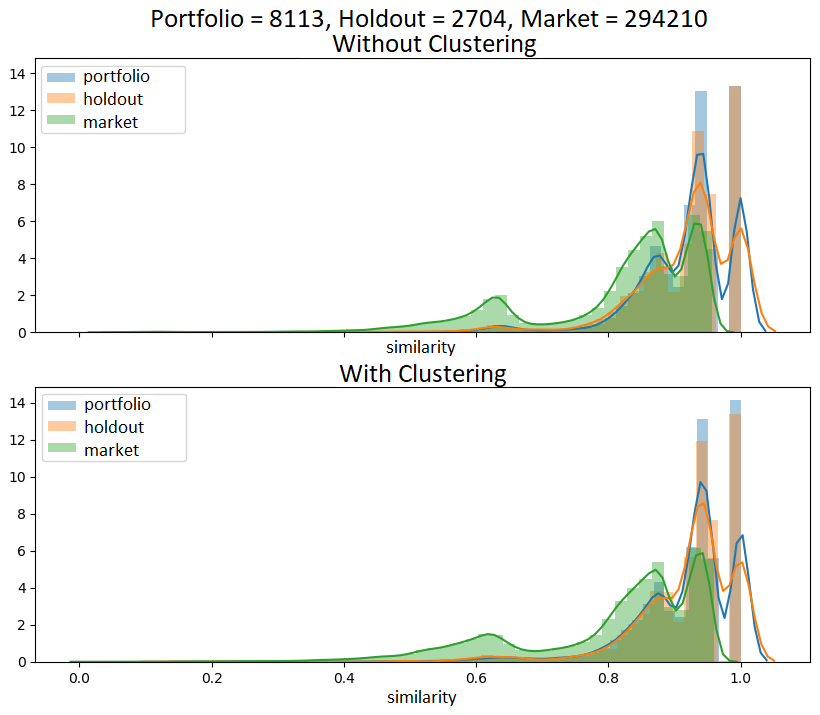
\includegraphics[width=7cm]{fig/ch4-bump-study-25.png}
   \caption{Similarity distribution plot for Study 25 on experiment \nameExperimentII{}. An example of study with multiple high density areas in the portfolio. Source: Author}
   \label{fig:bump-study-25}
\end{figure}

Study 25 is a study with a positive lift gain, that is, the performance of the study improved. However, looking at Figure \ref{fig:bump-study-25} we notice that the three modes of the portfolio distributions in the run without the clustering are preserved in the run with the clustering. We expected that each one of these peaks would shift to the right, close to similarity $1,0$. 

If we take a look at each clusters' similarity distributions plot we can see more clues for this behavior. Figure \ref{fig:study-25-clusters-simi-plot} shows these plots along with the clusters' sets sizes of the runs that did not had enough data. Figure \ref{fig:study-25-pca} shows its PCA plot with the portfolio and the market. 

\begin{figure}[!ht]
   \centering
   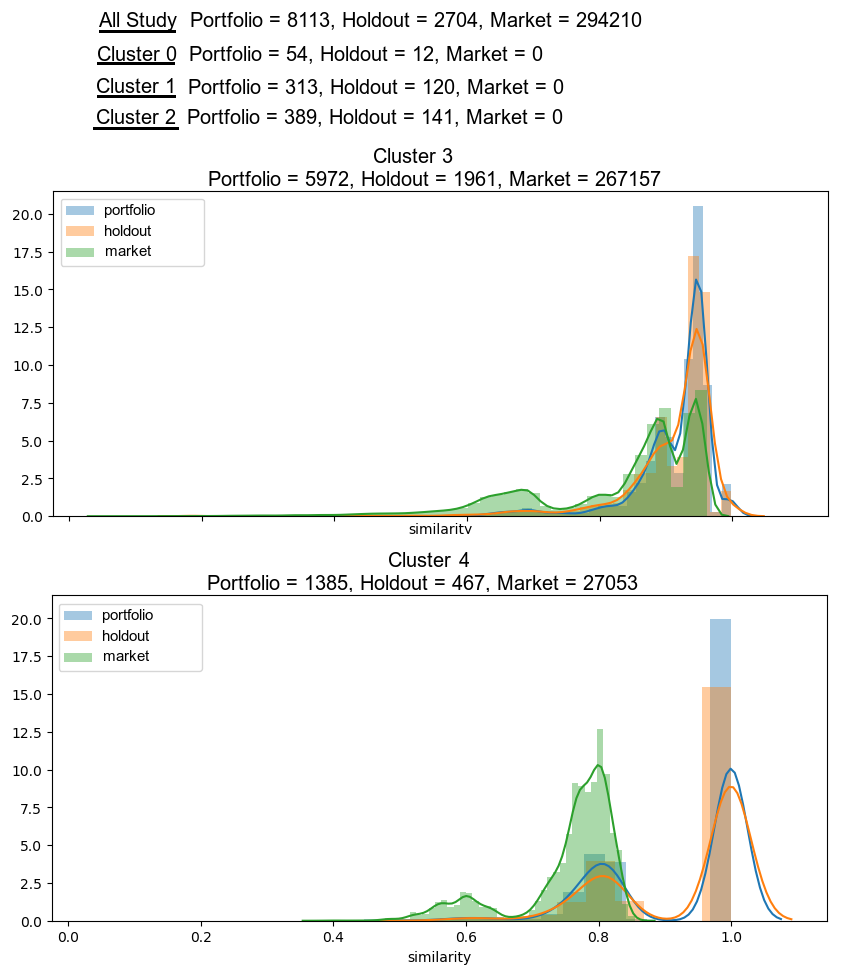
\includegraphics[width=8cm]{fig/ch4-study-25-clusters-simi-plot.png}
   \caption{Clusters' similarity distributions plots for Study 25 in experiment \nameExperimentI{}. Source: Author}
   \label{fig:study-25-clusters-simi-plot}
\end{figure}

There are five cluster in the portfolio, but only two (Cluster 3 and 4) had a matching pair with the market. In these cases we see that they did not present a "one peak area" in the portfolio. Cluster 4 has two peaks: one near similarity $1,0$ and the other near $0,8$, and Cluster 3 two close peaks near similarity $0,9$. The other clusters with not enough data (0, 1, 2), the portfolio and holdout sets correspond to approximately $10\%$ of the study portfolio size. This is a small portion of the data and it only affects \nameExperimentI{}, after all, in \nameExperimentII{} there is no cluster pairing, since this information is used as a feature.

\begin{figure}[!ht]
   \centering
   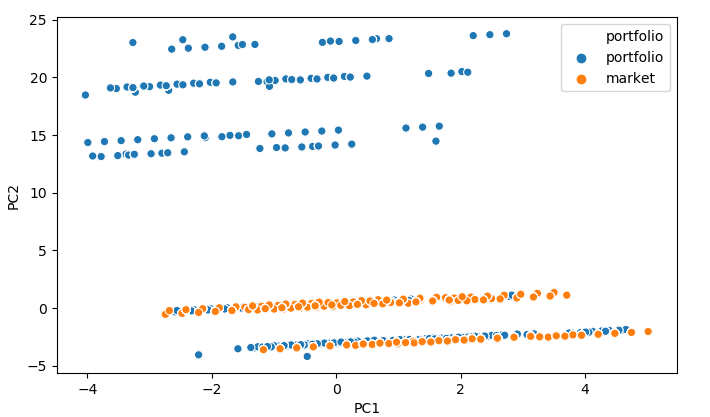
\includegraphics[width=8cm]{fig/ch4-study-25-pca.png}
   \caption{PCA plot with portfolio and market data for Study 25. Source: Author}
   \label{fig:study-25-pca}
\end{figure}

The outcome of these studies demonstrate that, perhaps, \textbf{our initial hypothesis is not on point}. There still other analysis to be done, such as, analyzing the companies from the similarity perspective, for instance, seeing what the companies in the high density area near similarity $0,9$ of some study have in common. These new perspectives emerged as the work was being developed. However, because of the time constraint, they could not be prioritized in this proof of concept. 

\subsection{Other relevant studies}
\label{ch:worth-ment}

There is another study that is not in one of the specifics lift-gain groups aforementioned, but its analysis of the similarity distribution is worth to be considered. Figure \ref{fig:worth-mentioning-study-7} shows the similarity distribution plots for Study 7 in the experiment \nameExperimentII{}. 

\begin{figure}[!ht]
   \centering
   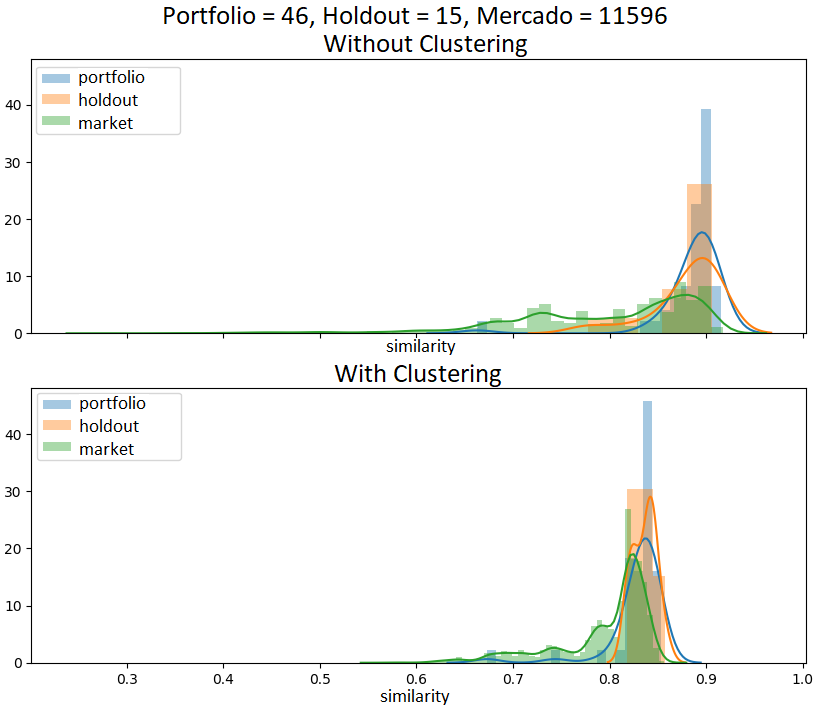
\includegraphics[width=8cm]{fig/ch4-worth-mentioning-study-7.png}
   \caption{Similarity distribution plot for Study 7 on experiment \nameExperimentII{}. Lift increased but the curves skewed to the left. Source: Author}
   \label{fig:worth-mentioning-study-7}
\end{figure}

This study had a lift gain of $12.5\%$, so its performance improved, thus the expected impact in the distributions is the holdout set increase its peak near similarity $1,0$ or to shift to this region when the distribution is located more on the left of the axis. Nonetheless, the opposite happens in this study. In Figure \ref{fig:worth-mentioning-study-7}, we see that the distributions keep its shape but shifted from similarity $1,0$ to around $0,85$. But since the holdout distribution stayed more in the right, in the first decile there are more companies from the holdout set, hence the increase on the lift

The cause of this shift was not investigated. But the main point of mentioning this study is to raise the awareness of the OT's team in the choice of metrics. This example indicate that only the lift is not enough to verify the output of the OT. As seen throughout section \ref{ch:simi-distis}, the lift and the similarity distribution plot are correlated, specially the distribution of the holdout set. Still, the lift is a metric of \underline{performance} and the similarity distribution plot shows the \underline{consistency} of the study. The shift of Study 7 was not critical, but if the similarity that the distributions went was $0,3$ instead of the $0,85$, the recommendations would not make sense for the OT's user due to its lack of consistency. That is why a new metric, that take into account consistency and performance, should be included in the overall benchmark of the studies.


\section{Experiment \nameExperimentII{} with other clustering algorithms}

The poor performance of the studies in experiment \nameExperimentI{}, which as the mean lift gain of $-9.871\%$, made the team of the OT to not proceed the testing of the clustering with this experiment. Although \nameExperimentII{} had a positive mean lift gain of $+2.016\%$, it was conducted with the "manual clustering". Thus, it was determined to oversee the results of this experiment with the other clustering algorithms previously presented in Figure \ref{fig:clustering-studies}. Figure \ref{fig:other-cluster-algo} shows the histogram of the lift gains of the re-runs for \nameExperimentII{} with KMeans (\ref{fig:other-cluster-algo:kmeans}), Gaussian Mixture (\ref{fig:other-cluster-algo:gmm}), and Bayesian Gaussian Mixture (\ref{fig:other-cluster-algo:bgm}).

\begin{figure}[!ht]
    \begin{subfigure}{.5\linewidth}
        \centering
        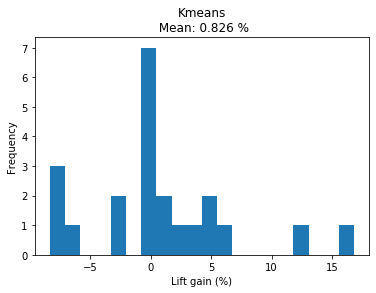
\includegraphics[width=5.5cm]{fig/ch4-kmeans_lift_gain_hist.png}
        \caption{}
        \label{fig:other-cluster-algo:kmeans}
    \end{subfigure}
    \begin{subfigure}{.5\linewidth}
        \centering
        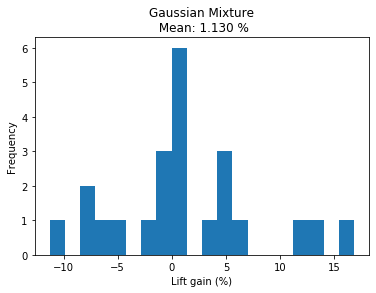
\includegraphics[width=5.5cm]{fig/ch4-gmm_lift_gain_hist.png}
        \caption{}
        \label{fig:other-cluster-algo:gmm}
    \end{subfigure}\\[1ex]
    \begin{subfigure}{\linewidth}
        \centering
        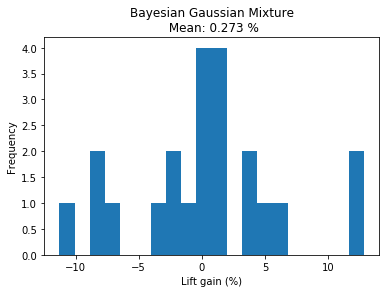
\includegraphics[width=5.5cm]{fig/ch4-bgm_lift_gain_hist.png}
        \caption{}
        \label{fig:other-cluster-algo:bgm}
    \end{subfigure}
    \caption{Lift gain histogram without outliers of other clustering algorithm runs for experiment \nameExperimentII{}}
    \label{fig:other-cluster-algo}
\end{figure}

We notice that none of them reached the lift gain of the "manual clustering". The closest one was the Gaussian Mixture with $1.13\%$. The other two resided below $1\%$ ($0.8$ for KMeans and approximately $0.3$ for Bayesian Gaussian Mixture). The outcome of these results consolidate the strategy of cluster the studies manually, meaning that the groups in the PCA plots make sense, at least in the performance perspective of the OT. 

Despite of this confirmation on the strategy adopted by the team, this is not feasible for the OT, since it is impossible to the system run in production with human interference during the leads scoring. The clustering done manually could be use as a success criteria for other clustering algorithms, but that would turn the type of problem to a classification, due to the presence of the labels.

Another alternative to improve the performance in experiment \nameExperimentII{} without the manual clustering, is to tweak the hyper-parameters of the Gaussian Mixture and see if it the lift gain approaches the achieved mark of $2\%$. For instance, in the Scikit-learn Python package, this algorithm has up to seven different hyper parameters that go from initialization, weights settings up to convergence settings \cite{scikit-learn}.